\section{Approach}

\subsection{Algorithm}

\begin{frame}{MABDI Algorithm} % _______________________________________________
  \vspace{-0.13in}
  \includegraphics[height=0.95\textheight]<1>
    {../figures/presentation/approach_mabdi_algorithm_p0.pdf}
  \includegraphics[height=0.95\textheight]<2>
    {../figures/presentation/approach_mabdi_algorithm_p1.pdf}
  \includegraphics[height=0.95\textheight]<3>
    {../figures/presentation/approach_mabdi_algorithm_p2.pdf}
  \includegraphics[height=0.95\textheight]<4>
    {../figures/presentation/approach_mabdi_algorithm_p3.pdf}
  \includegraphics[height=0.95\textheight]<5>
    {../figures/presentation/approach_mabdi_algorithm_p4.pdf}

    \note<1>{\begin{itemize}
      \item[] System diagram of the MABDI algorithm
      \item[] Orange -
      \item Input to the algorithm
      \item has been simulated for this work.
      \item[] Classification -
      \item These components are what make MABDI unique
      \item They classify data before it is added to the Global Mesh.
    \end{itemize}}

  \note<2>{\begin{itemize}
    \item[] Input
    \item I will cover simulation process in the next section.
    \item[] Generate Expected Depth Image
    \item Takes the global mesh (what we know about the environment)
    \item And pose of sensor.
    \item Generates what we expect to see.
    \item Meaning what would a RGB-D sensor would see.
    \item Given what we know about the environment and the pose of the sensor.
  \end{itemize}}

  \note<3>{\begin{itemize}
    \item[] Classify Depth Image
    \item This is the heart of MABDI
    \item and is MABDI's contribution to the state-of-the-art
    \item It determines which points from D are novel.
    \item (From a new part of the environment that has not been seen before)
    \item Taking the absolute difference between $E$ and $D$ and thresholding.
    \item (point to equation)
    \item If the differences are small, those points are thrown away.
    \item If the differences are large, those points are kept.
    \item If the difference is large, the measurements are coming from a part of the environment that has not been seen before.
  \end{itemize}}

  \note<4>{\begin{itemize}
    \item[] Surface Reconstruction
    \item Create a mesh structure from the novel points
    \item Cover in detail next
  \end{itemize}}

  \note<5>{\begin{itemize}
    \item Add Novel Surface to Global Mesh
    \item Append surface to the global mesh
    \item that is continuously being updated
  \end{itemize}}

\end{frame}


\subsection{Surface Reconstruction}

\begin{frame}{Initial Mesh} % __________________________________________________
  \only<1>{
    Surface Reconstruction component is responsible for creating the novel surface $S$ from the novel points $D_n$ \\ \medskip
    Our Method:
  \begin{itemize}
    \item Define topology in 2D, on the depth image
    \item Project to 3D
    \item Remove elements
  \end{itemize}}

  \begin{center}
    \includegraphics[height=0.90\textheight]<2>
      {../figures/approach_sr_topology.pdf}
  \end{center}

  \includegraphics[width=\textwidth]<3>
    {../figures/presentation/approach_project_p.pdf}

  \note<1>{\begin{itemize}
    \item I just described the MABDI algorithm
    \item The algorithm is simply an idea
    \item I am going to describe how I implemented this idea
    \item[]
    \item topology or structure
  \end{itemize}}

  \note<2>{\begin{itemize}
    \item Imagine this is the depth image
    \item - Every blue point is a pixel in the depth image
    \item - Corresponds to 3D point in space
    \item Depth image
    \item - Not a set of unorganized points
    \item - Has structural information
    \item - This allows us to define a topology in 2D that is preserved when projected to 3D
    \item I then take every blue dot and project them into 3D space
    \item preserving the connections between vertices
  \end{itemize}}

  \note<3>{\begin{itemize}
    \item Imagine mesh being defines using every pixel in depth image
    \item Then projected to 3D space
    \item - Ignore the background for now
    \item Note there will be no surface
    \item behind the cup,
    \item under the table,
    \item anywhere on the floor that the sensor doesn't see
  \end{itemize}}
\end{frame}


\begin{frame}{Removing elements} % _____________________________________________
  \begin{center}
    \only<1>{
      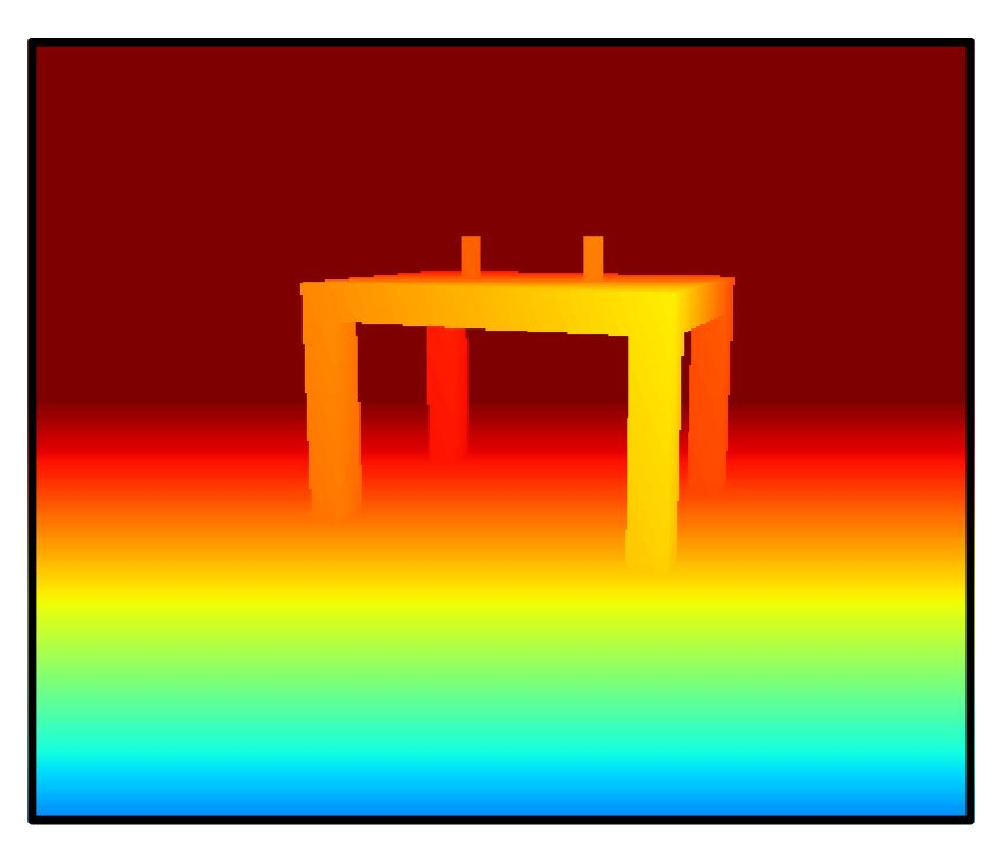
\includegraphics[height=0.90\textheight]
        {../figures/presentation/approach_depth_image_p.pdf}
    }
    \only<2>{
      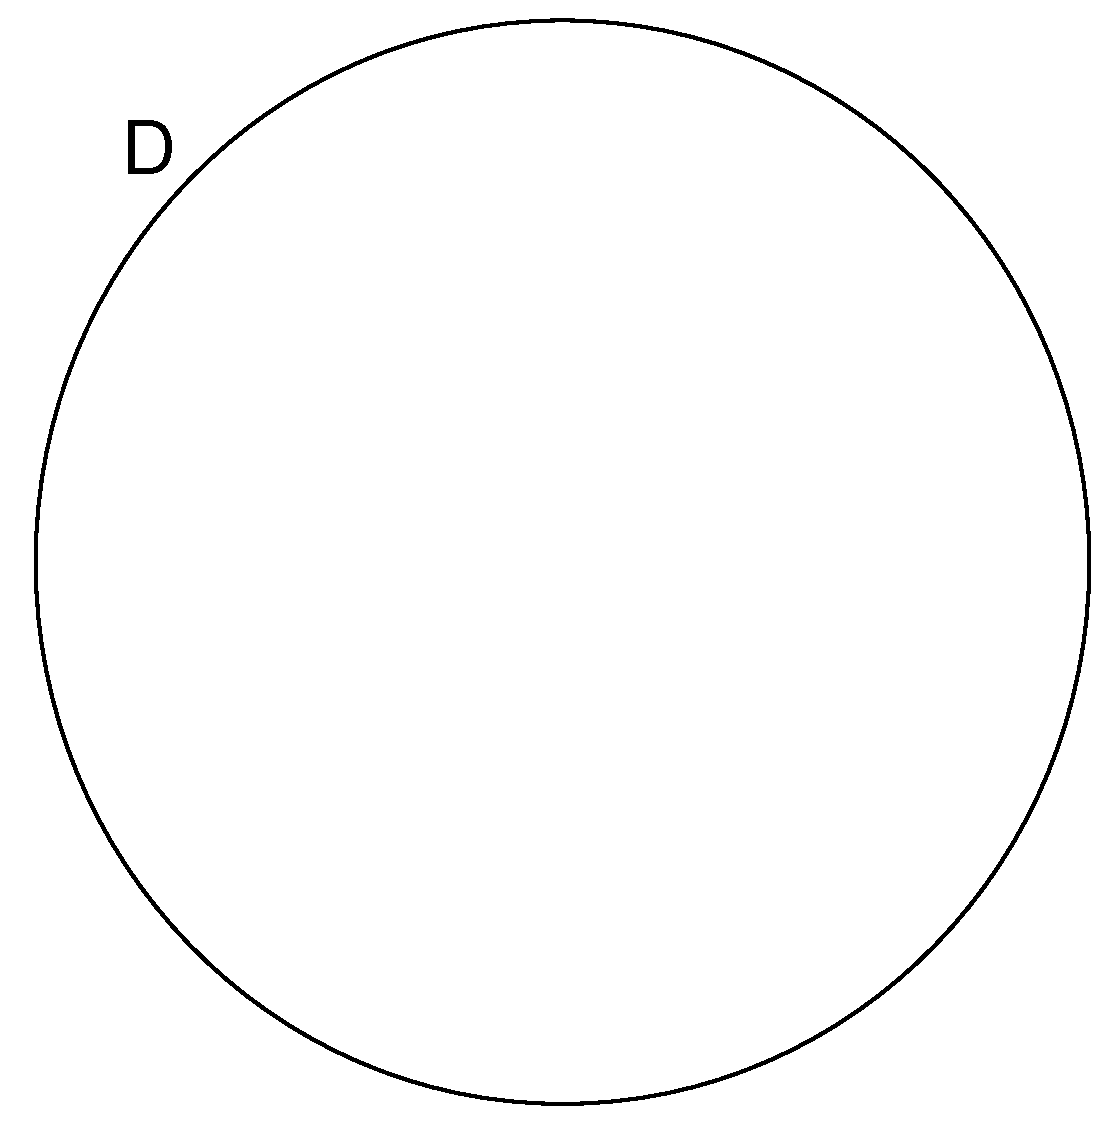
\includegraphics[height=0.65\textheight]
        {../figures/presentation/approach_sr_pts_0.pdf}
    }
    \only<3>{
      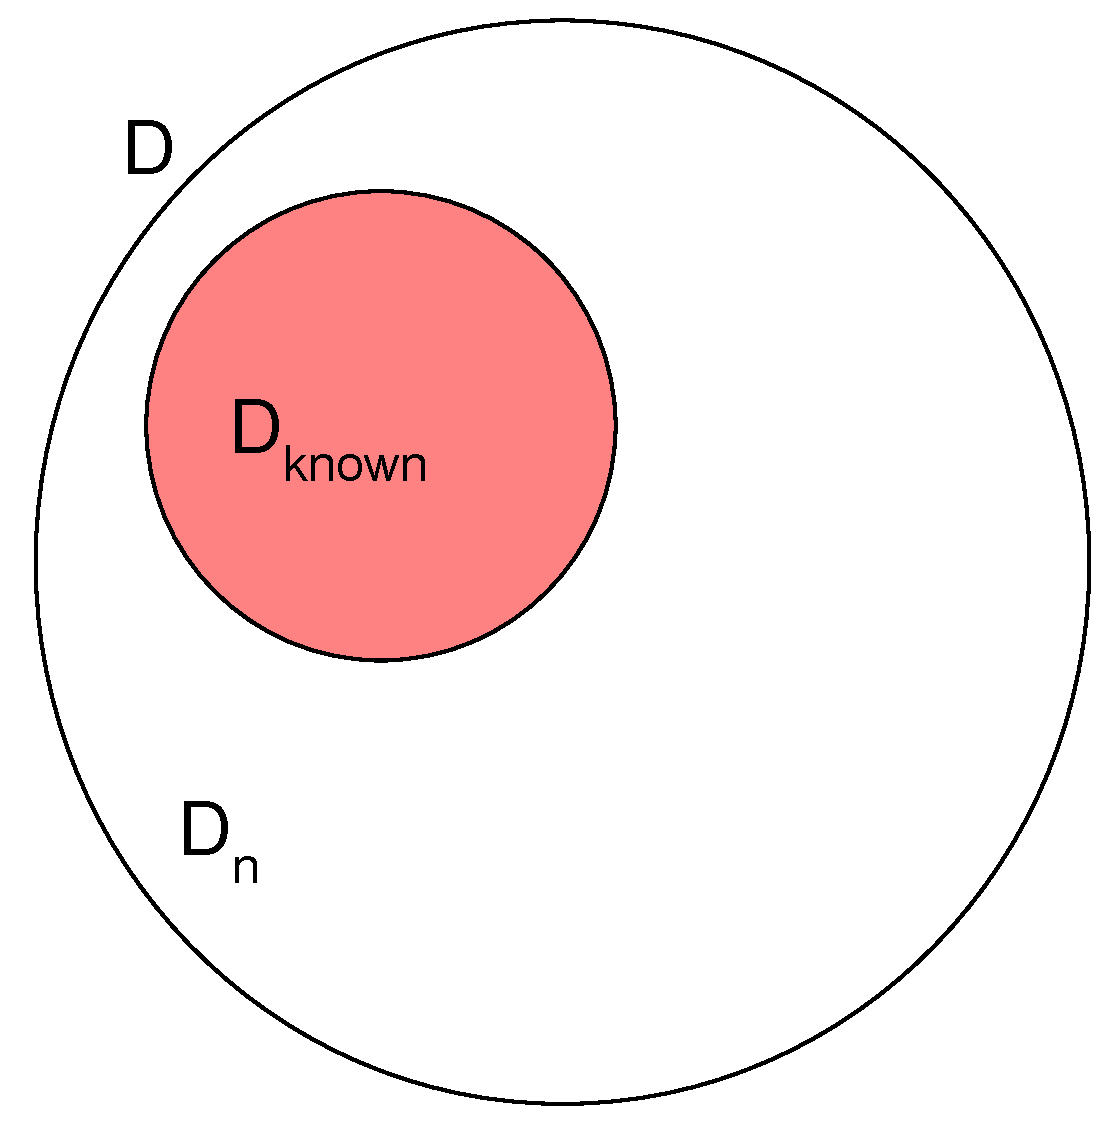
\includegraphics[height=0.65\textheight]
        {../figures/presentation/approach_sr_pts_1.pdf}
      \begin{gather*}
        D_n = \lvert D - E \rvert > threshold \\
        D_{known} = D \setminus D_n
      \end{gather*}
    }
    \only<4>{
      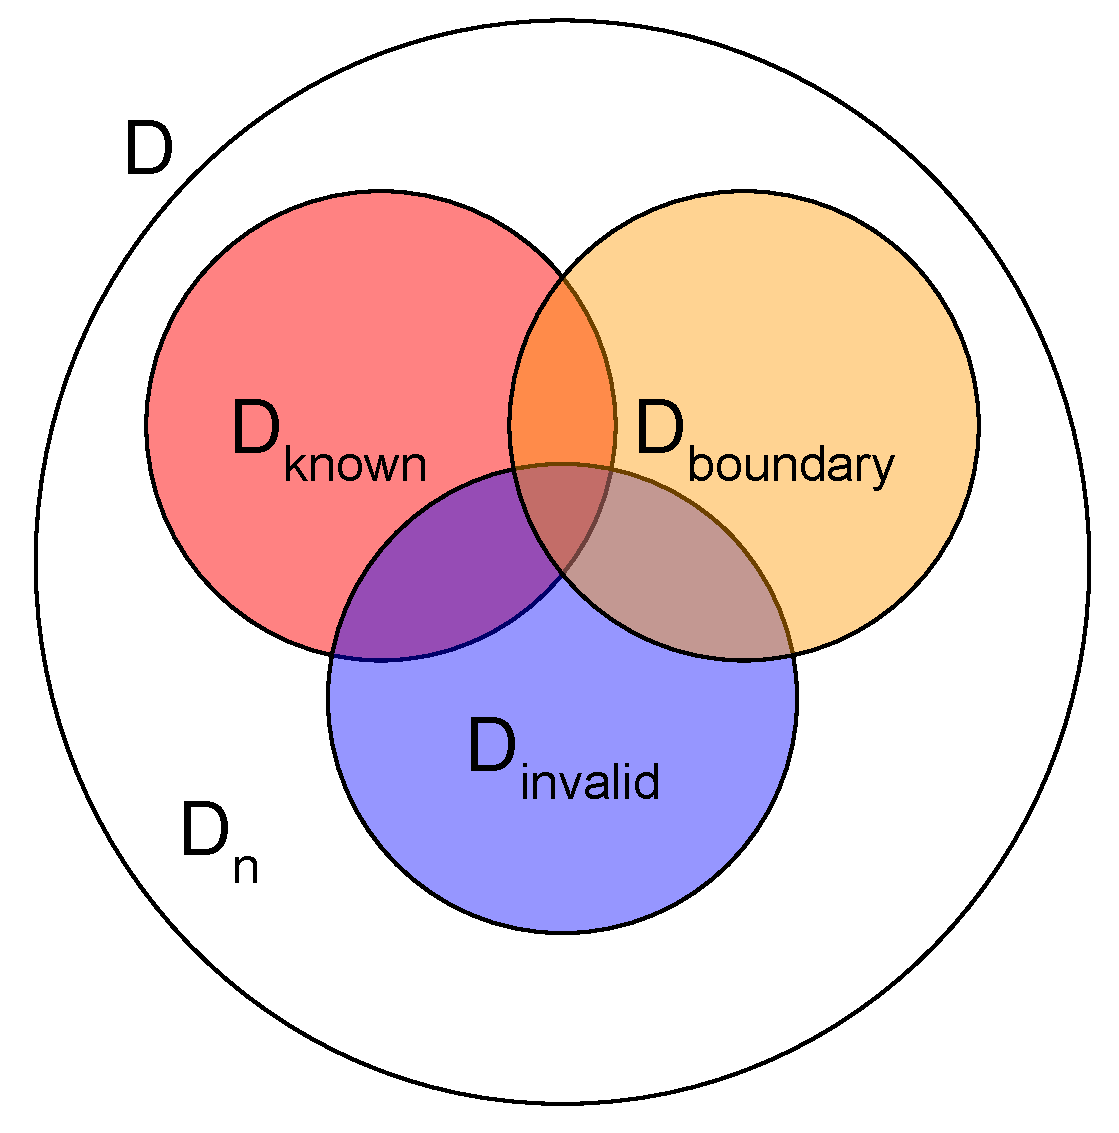
\includegraphics[height=0.65\textheight]
        {../figures/presentation/approach_sr_pts_2.pdf}
      \begin{gather*}
        K = \begin{bmatrix} 2 & -1 \\ -1 & 0 \end{bmatrix} \\
        D_{boundary} = (D \ast K) > threshold
      \end{gather*}
    }
\end{center}

  \note<1>{\begin{itemize}
    \item I begin removing elements by first identifying
    \item[] points to be removed from the depth image
  \end{itemize}}

  \note<2>{\begin{itemize}
    \item Inside the circle represents every point from $D$
  \end{itemize}}

  \note<3>{\begin{itemize}
    \item $D_n$ (novel) is the set of points that the categorization process said is novel
    \item Categorization process is defined by this equation
    \item[] absolute difference between what the sensor saw and what we expect to see
  \end{itemize}}

  \note<4>{\begin{itemize}
    \item I define two additional set of points to be thrown away.
    \item $D_{boundary}$
    \item - remove elements defined by points that lie on completely different surfaces
    \item - pixel neighbors floor and leg (point out difference in values)
    \item - To achieve this a two dimensional, differencing convolution filter is passed over $D$
    \item - Filter has a magnified response at points where the difference
    between neighboring pixels is large
    \item $D_{invalid}$
    \item - elements that are out of range of the sensor
  \end{itemize}}
\end{frame}

\begin{frame}{Removing elements} % _____________________________________________
  \begin{center}
    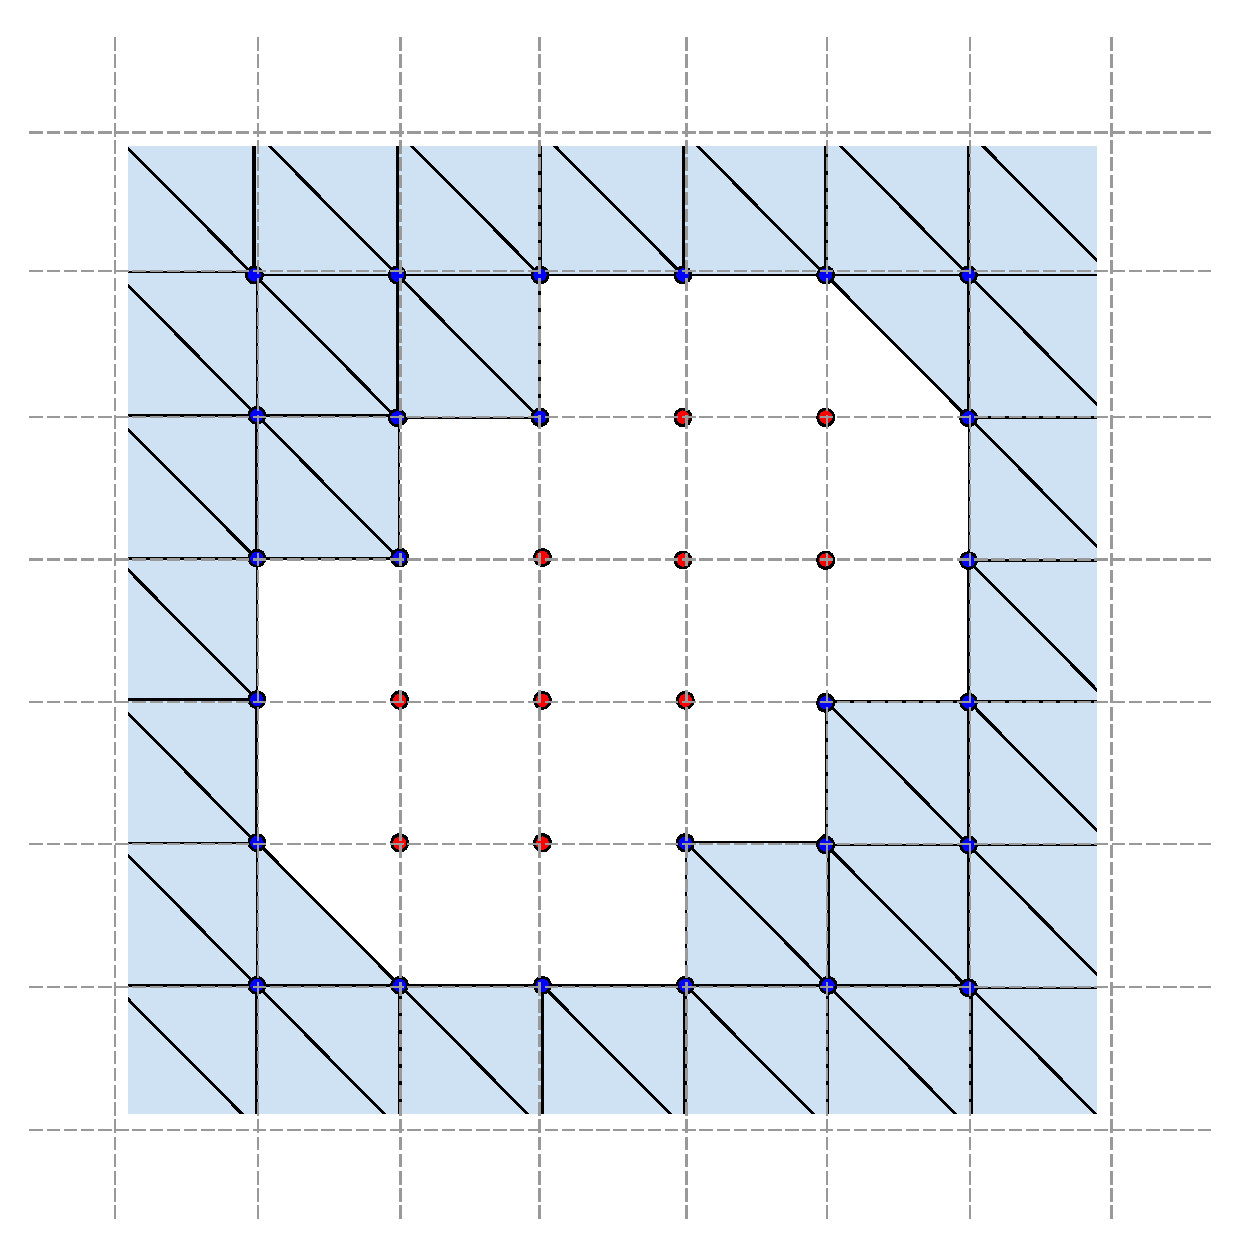
\includegraphics[height=0.90\textheight]
      {../figures/approach_sr_element_removal.pdf}
  \end{center}
  \note{\begin{itemize}
    \item Points from the colored circles are represented as the red points
    \item []
    \item Technically, these points have already been projected to 3D
    \item but this is the best way to visualize this concept
  \end{itemize}}
\end{frame}
